%========= Introduction
\section{Introduction}~\label{sec:introduction}
\subsection{Aim \& Objectives}~\label{subsec:aims}

\begin{figure}[h]
    \centering
    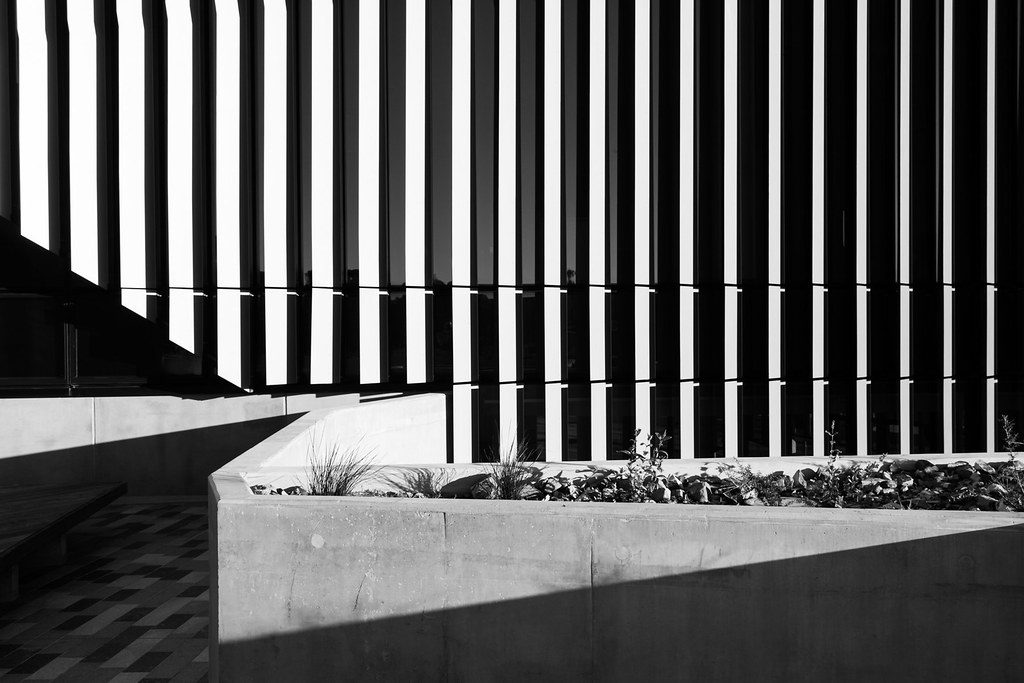
\includegraphics[width=0.7\textwidth]{Deakin_img.jpg}
    \caption{Deakin Campus Building.}
    \label{fig:building}
\end{figure}

Figure~\ref{fig:building} shows the Deakin BC building at Burwood campus in Melbourne.

\subsection{Structure}~\label{subsec:structure}
Section~\ref{sec:literature} reviews the literature. Section~\ref{sec:design} presents the research design and methodology. Section~\ref{sec:approach} describes the approach and the technical details of artefact development. Section~\ref{sec:evaluation} evaluates the artefacts, on the basis of research questions (RQs) in Section~\ref{subsec:RQs} and discusses the RQs in Section~\ref{sec:discussion}. Section~\ref{sec:threats} discusses threats to validity and Section~\ref{sec:conclusion} concludes the report. 

What is Iot?
The Internet of Things (IoT) has revolutionised the way devices are connected and interconnected in today's modern world. In a smart home, you can control every electronic appliance from your mobile phone and know what is happing both inside and outside of your home without being there. For example, a smart fridge would allow you to see the inside of your fridge, control its thermostat, automatically add a finished item to a purchase list and even order it for you if needed. The Internet of Things (IoT) consists of over a billion devices connected to the internet worldwide today, the types of devices increase daily. With the introduction of 5G internet, different studies conducted estimate by the year 2025, 75 billion IoT devices will be connected to the internet.

What is a Public Camera?
A Public Camera is also known as a Public Smart Camera; it is an advanced surveillance camera mounted and used by law enforcement and authorities. This camera's purposes could be to detect; traffic, disruptions, people falling, incidents, fires, speeding vehicles, recognise objects, recognise emotions, and other surveillance-related options. Through these cameras, people feel a greater sense of safety, and the trend is that fewer crimes are committed. Some of these cameras also feature Pan Tilt Zoom (PTZ), a technology giving the ability to move these cameras 360 degrees and see what is happening all around the camera. The camera can remotely be controlled with the tilt allowing the camera operator to move the camera lens up and down, and the zoom features allow the operator to focus on a particular area or location. As Sydney slowly becomes a smart city, we see PTZ cameras mounted on every primary traffic light and intersection.
 
What is a Civilian Drone?
The term drone originates from the military and means un-manned ariel vehicle in otherwords a crewless vehicle with a pre-programmed route.  Since the beginning of 2000, flying toys have increased; we first saw flying helicopters and then the introduction of what looked like a flying dish and then the mini quadcopter.  From 2010 on wards, the shape of these toys improved, and the result is what we see now as flying drones. Civilian drones do not have any weapons attached and are used by, recreationists, bloggers, videographers, photographers, delivery companies and many others.  The drone is also an aircraft that is controlled remotely, working together with onboard sensors and different GPS technology. Drones are made from very strong and light material, allowing easy manoeuvring and a reliable flight. Drones can fly to very high altitudes and can be programmed to take off, fly a certain route, deliver an item and then come back. Civilian Drones today either have a 4K camera built into the drone, or allow the addition of a 4K action camera such as a GOPro. Simillarly to a PTZ camera, you are able to maneuver the camera as well as the drone, most drones allow you to view the camera remotely VIA your mobile or via the wireless controller. For a higher quality recording, there is an SD card on the device that also acts as a secondary backup. 
